\section{Løsningsbeskrivelse}

Som løsning til problemstillingen er der fremstillet et website (Converge-SPA) \cite[Converge-SPA]{converge-terms}, der gør det muligt at købe og sælge arbejdskraft, mellem henholdsvist employer og freelancer. Til websitets koncept er der taget inspiration fra andre lignende sites, såsom Fiverr.com, Freelancer.com, worksome.dk osv. \cite[Inspiration sites]{converge-terms}. Dog er der med Converge mere fokus på samarbejde og kommunikation end disse platforme. Desuden er Converge fremstillet til at være så fremtidssikret som muligt, og bruger det nyeste men stadig modne teknologi, for at brugeren får den mest behagelige oplevelse.

En given bruger kan være freelancer, employer eller begge dele. Selve forløbet starter med at en employer opretter et projekt, efter eget ønske. Til at starte med kan employeren definere en pris og indsætte en beskrivelse, samt uploade nogle filer til at forklare hvad personen gerne vil have lavet.

En freelancer kan derefter vælge at lægge sit bud og en kommentar på dette projekt, og employeren kan efterfølgende vælge at acceptere buddet, eller tage en dialog med freelanceren. Efter at freelanceren er valgt kan projektet starte, employeren fortæller freelanceren hvad der ønskes lavet og freelanceren har nu mulighed for at spørger om alle de detaljer der skal til. Dette kunne være enten at bruge de interne projektsamarbejdsværktøjer eller ved at føre en dialog over tekst- eller videochat.

Freelanceren kan nu arbejde på projektet og indlevere sit materiale i iterationer, for at få employerens kommentar og meninger. Hvis employeren siger god for det, så vil freelanceren anmode om betaling i bytte for det materiale personen/firmaet har fremstillet.

Employeren får en anmodning om at betale. Hvis det vælges, så vil employeren modtage resultatet af projektet og freelanceren kan modtage betaling for det arbejde der er blevet gjort.

Til at klare dette er der brug for funktionalitet til at have brugere, projekter, tekstchat, betaling, osv.

Dette er løst ved at dele projektet op i 2 dele; en webapplikation (Converge-SPA) og en backend (Converge-cluster) \cite[Converge-cluster]{converge-terms}.

\begin{figure}[H]
  \begin{small}
    \begin{center}
      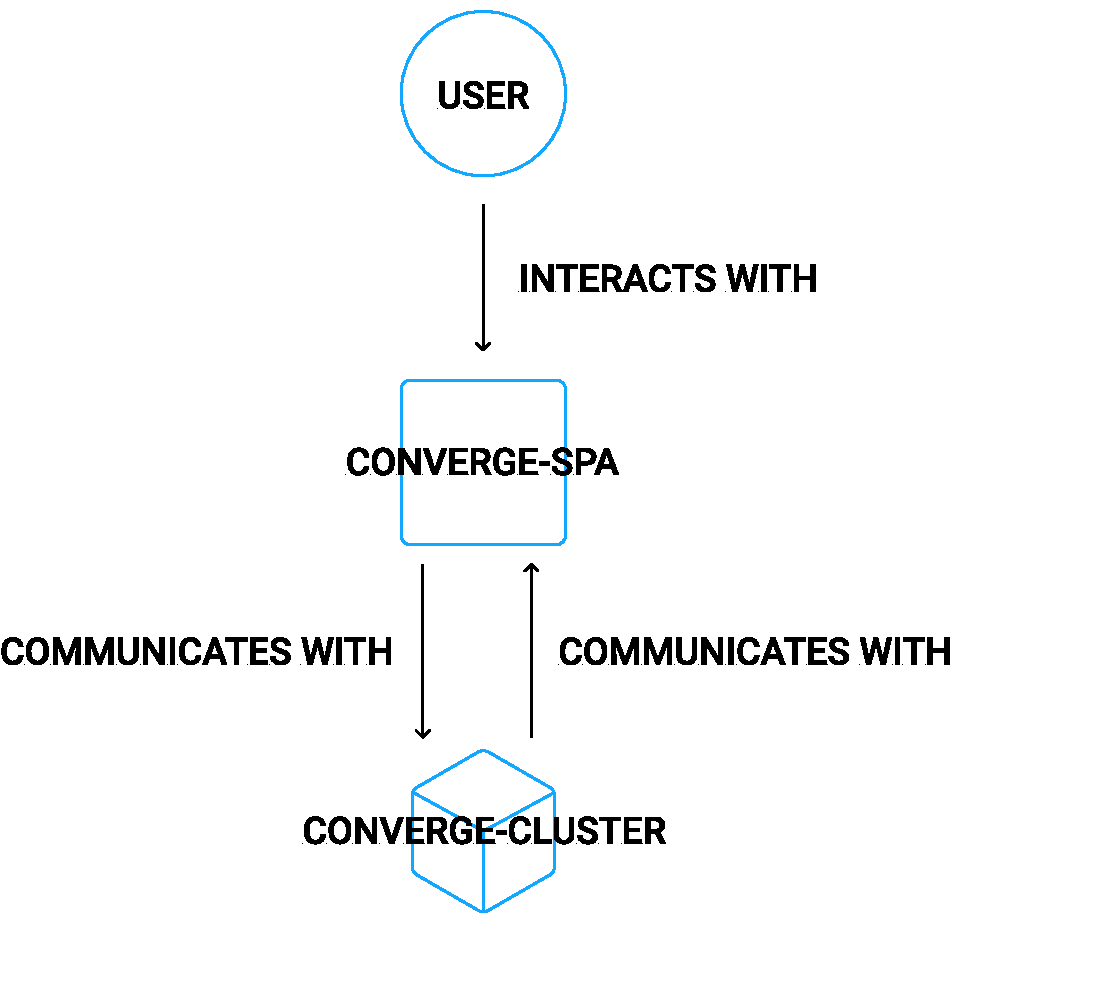
\includegraphics[width=0.45\textwidth]{Billeder/Architecture.pdf}
    \end{center}
    \caption{Overblik over arkitektur}
    \label{fig:simple-architecture}
  \end{small}
\end{figure}

Converge-SPA er det som brugeren ser og interagere med, hvis webgrænsefladen er valgt. Hvis ikke, tilbyder Converge-cluster et API \cite[API]{converge-terms} som kan det samme. Converge-cluster er der hvor al logik hører hjemme, det er kernen af produktet og indeholder alle de services der udgøre produktet Converge \cite[Converge]{converge-terms}. Converge-cluster sørger for alt fra web-servere til databaser, load-balancing, monitorering og meget mere.